\documentclass[]{article}
\usepackage{graphicx}
\usepackage{rotating}
\usepackage{apacite}
\usepackage[numbib]{tocbibind}

%opening
\title{Maximum entropy and population heterogeneity in continuous cell cultures meet experimental data, preliminary results}
\author{}

\begin{document}
	
	\maketitle
		
	\section{Materials and Method}
	
	%%%%%%%%%%%%%%%%%%%%%%%%%%%%%%%%%%%%%%%%%%
	%%%%%%%%%%%%%%%%%%%%%%%%%%%%%%%%%%%%%%%%%%%%%%%%%%%%%%%%%%%%%
	\subsection{Model framework }
	
	The model framework used is detaily explained in \cite{Fernandez-de-Cossio-Diaz2017} and \cite{Fernandez-de-Cossio-Diaz2018b}
	
	\subsection{Experimental data} %%%%%%%%%%%%%%%%%%%%%%%%%%%%%%%%%%%%%%%%%%
	
	Experimental data was taken from \cite{Rath2017a}, in this work the author performed 6 continuous cultures, ($A$, $B$, $C$, $D$, $E$, $F$), with the cell line AGE1.HN.AA1, which parental line AGE1.HN was established by the company ProBioGen (ProBioGen AG, Berlin, Germany) from a tissue sample of a human brain. All culture's feed mediums was based on the standard 42-Max-UB-medium, which is serum-free and was specially developed for the AGE1.HN cell line $Table 1$. The experiments were run under various conditions, differing mainly in the dilution rate ($D$) and the feed medium composition of glucose ($GLC$), glutamine ($GLN$) and galactose ($GAL$) $Table 2$. \\
	For each experiment, a steady-state condition was reached, ($A$, $B$, $C$, $D$, $E$, $F01$), and several observables  was reported $Tables 3-4$. Particularly relevant for this work was the growth rate ($\mu$), $D$, the viable cell density ($Xv$) and the medium concentration ($s$) and derived uptake rate ($u$) for a set of metabolites ($GLC$, lactose ($LAC$), $GLN$, ammonium ($NH4$), $GAL$, pyruvate ($PYR$), glutamate ($GLU$), alanine ($ALA$), asparagine ($ASP$)). A unit conversion was required to make experimental data and models compatible. For this propose the only external data needed was the cell mass density. It was used  0.25 pgDW/ $\mu$$m^3$ \cite{Niklas2010}.
	
	\subsection{Preparing GEMs} %%%%%%%%%%%%%%%%%%%%%%%%%%%%%%%%%%%%%%%%%%%
	
	In order to preliminary evaluate the capacity of the model to reproduce the experimental data, two Genome-scale Metabolic Models ($GEM$) was prepared.
	
	\subsubsection{Recon3D}
	
	Recon3D represents the most comprehensive human metabolic network model to date \cite{Brunk2018}. The model,
	Recon3DModel\_301.mat, was downloaded from http://vmh.life. The original biomass equation was modified to adjust the biomass demand reported by $Niklas$ for the parental line AGE1\_HN. All the other original demands from recon3D were deactivated. An extra demand representing the maintenance demand, not associated with growth, of atp was set according to \cite{Fernandez-de-Cossio-Diaz2018b}. All the fluxes representing exchangeable metabolites (external reactions) were set as reversible (lb and ub set to a large number), so the only effective bound constraints (for FBA and EP) are the ones produced by the chemostat consideration \cite{Fernandez-de-Cossio-Diaz2018b}. Additionally, for including the molecular crowding constraints we map $Shlomi$ enzymatic costs, initially defined for recon1, to recon3D.\\
	Pursuing to reproduce the conditions of the different steady states, the external concentrations of the exchangeable metabolites were set using the data from $Tables 1-2$. Additionally, external concentrations of salts, oxygen, and other metabolites not specified in the medium were set to a large number. Particularly, Recon3D was unable to grow without pe\_hs[e], phosphatidylethanolamine, (or similar) lipid in the feed medium. Later we will discuss the impact of this metabolite in the medium.  
	
	\subsubsection{CHO}
	
	Chinese hamster ovary (CHO) host cell-lines GEM was obtained from \cite{Hefzi2016a} and was setup as \cite{Fernandez-de-Cossio-Diaz2018b}.  The external metabolite concentrations were set to the values indicated in $Table 1-2$, similar to Recon3D. Also, a few extra metabolites, taken from \cite{Fernandez-de-Cossio-Diaz2018b} was included in the feed medium. An important different from Recon3D was that CHO is able to grow without pe\_hs[e], named in CHO as pe\_cho\_e. 
	
	
	
	\section{Results} %%%%%%%%%%%%%%%%%%%%%%%%%%%%%%%%%%%%%%%%%%%%%%%%%%
	%%%%%%%%%%%%%%%%%%%%%%%%%%%%%%%%%%%%%%%%%%%%%%%%%%%%%%%%%%%%
	
	\subsection{Low concentrations of phosphatidylethanolamine} %%%%%%%%%%%%%%%%%%%%%%%
	
	Because phosphatidylethanolamine isn't a reported component of the 42-Max-UB-medium $Tabla\ 1$ and it can be a carbon source for the GEMs, its concentration was set first to the lowest value possible. For Recon3D it was fixed to 0.1mM, a handpicked value, and for CHO it wasn't present in the feed medium at all.\\ 
	Flux balance analysis with molecular crowding (FBAwMC) was performed similarly to $Cossio$. Plots of $\mu$ and $Xv$ as function of $\xi$ are shown in $Figure\ 1$. As can be appreciated from the comparison of the model prediction (solid lines) with the experimental data (colored circles), FBAwMC have a big problem reproducing both observables. Especially for $Xv$, the predictions was really far from the expected, never reaching a high enough value.\\
	The correlations of the experimental and the modeled uptakes, $Figure\ 2$, show better results for CHO. This could be, maybe, explained because Recon3D is a general GEM, allowing access to all the possible genome repertory present in humans, a fact that is not accurate for a cell in a $in\ vivo$ scenario. On other hand, CHO was curated for a defined cell line, representing a more restricted and realistic network. Anyway, it is remarkable how the models reproduce uptakes like $GLC$ and $GLN$ regarding the previous consideration.
	
	\subsection{High concentrations of phosphatidylethanolamine} %%%%%%%%%%%%%%%%%%%%%%%
	
	% Bibliography!!!!
	\bibliographystyle{apacite}
	\bibliography{/Users/Pereiro/Documents/library.bib}
	
	% Tables and Figures
			\begin{table} % Table 1
		\centering
		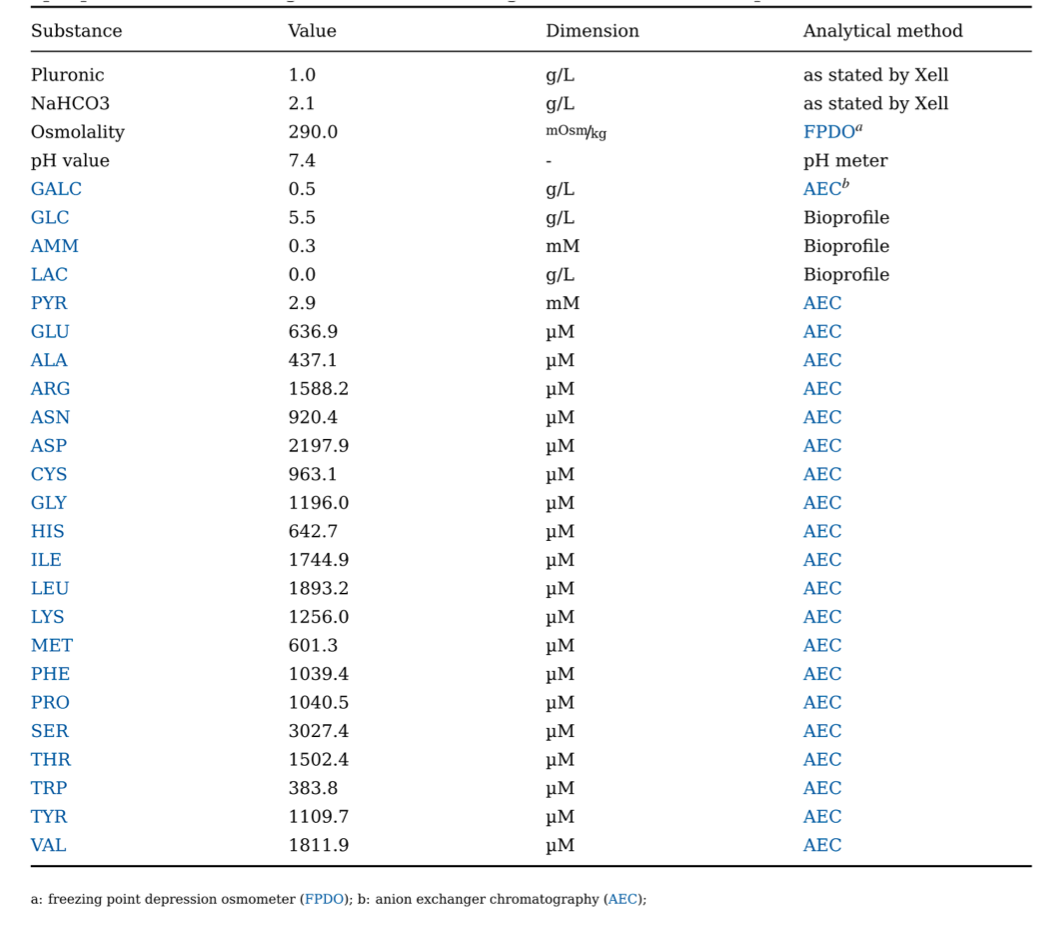
\includegraphics[scale = 0.68]{Table_3_1}
		\caption{Measured medium composition of the 42-MAX-UB standard medium. Extracted from \protect\cite{Rath2017a}}
		
	\end{table}
	
	\begin{table} % Table 2
		\centering
		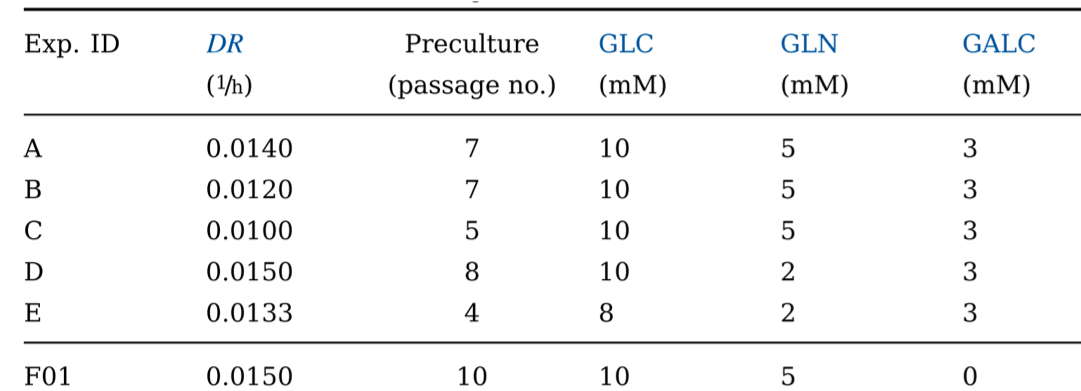
\includegraphics[scale = 0.63]{Table_4_10}
		\caption{The dilution rates, preculture ages and the 42-Max-UB-medium modified components concentrations used in \protect\cite{Rath2017a} for the 6 steady states. Table adapted from \protect\cite{Rath2017a}}
		
	\end{table}
	
	\begin{sidewaystable} % Table 3
		\centering
		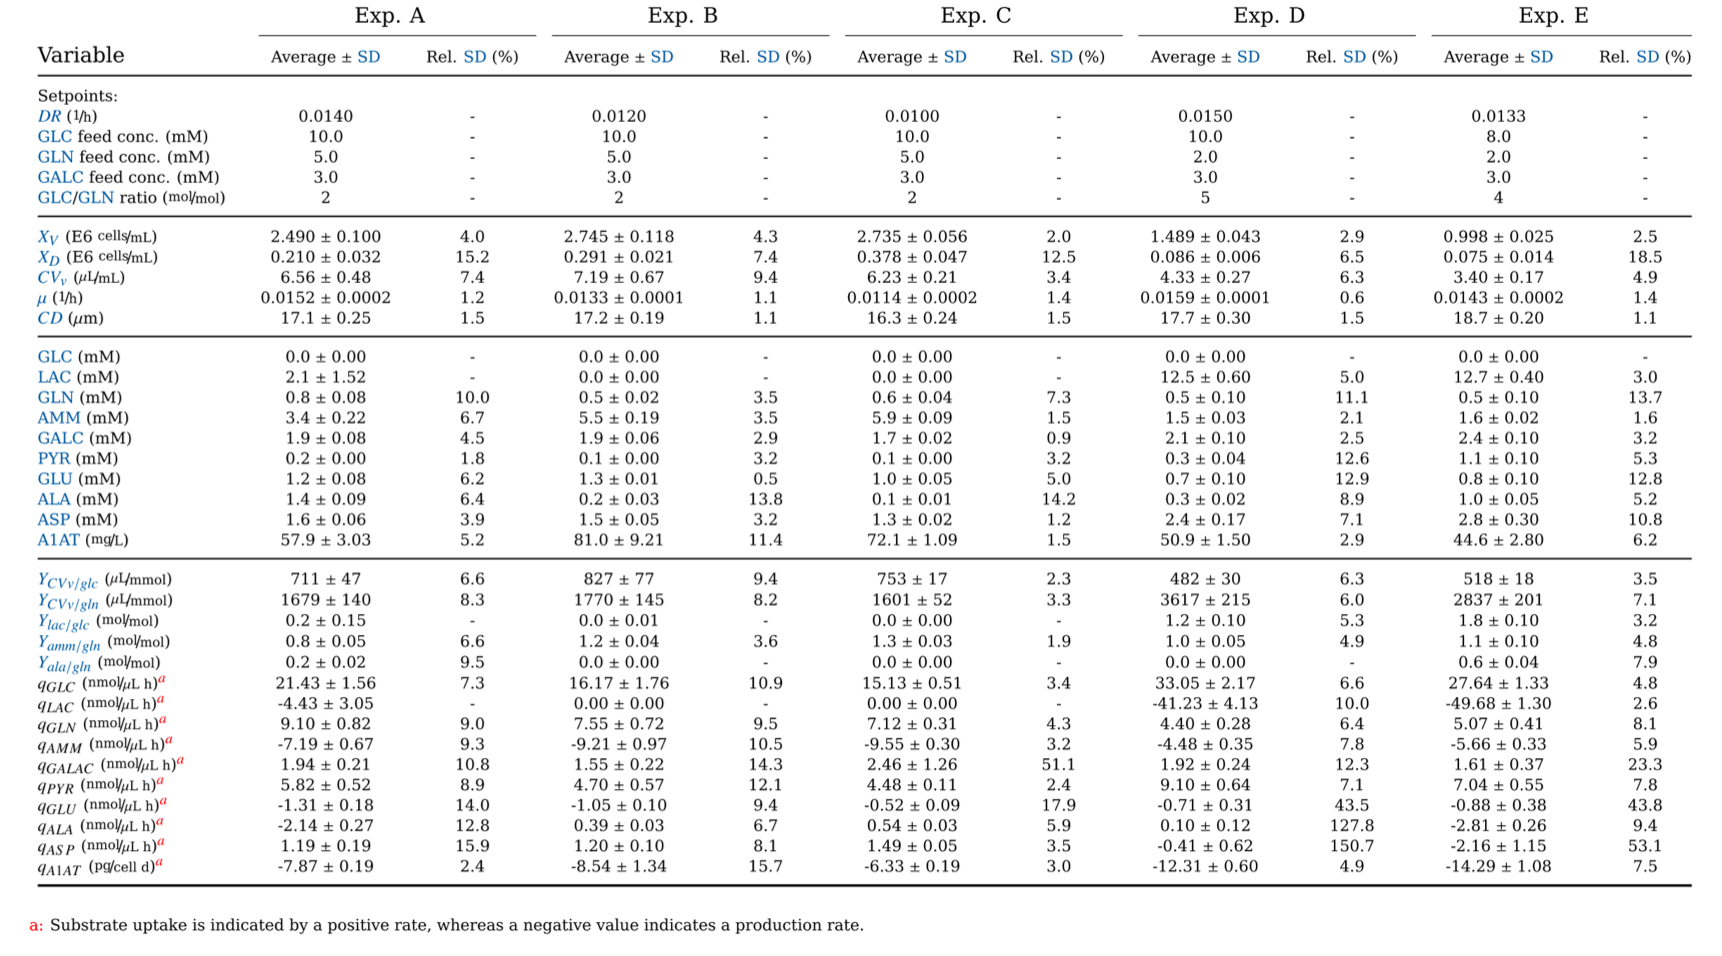
\includegraphics[scale = 0.7]{Table_4_11}
		\caption{Steady-state values reported for \protect\cite{Rath2017a} of different parameters from continuous cultivations with varying GLC and GLN feed concentrations and with 3 mM GAL. Table taken from \protect\cite{Rath2017a}}
		
	\end{sidewaystable}
	
	\begin{table} % Table 4
		\centering
		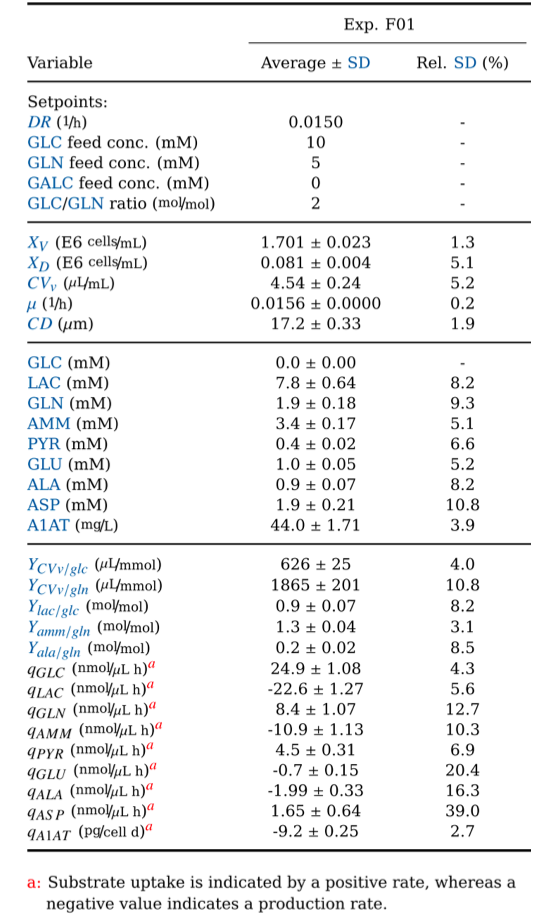
\includegraphics[scale = 0.8]{Table_4_12}
		\caption{Steady-state values reported for \protect\cite{Rath2017a} of different parameters from continuous cultivations with varying GLC and GLN feed concentrations and without GAL. Table taken from \protect\cite{Rath2017a}}
		
	\end{table}
		\begin{figure}[h]
		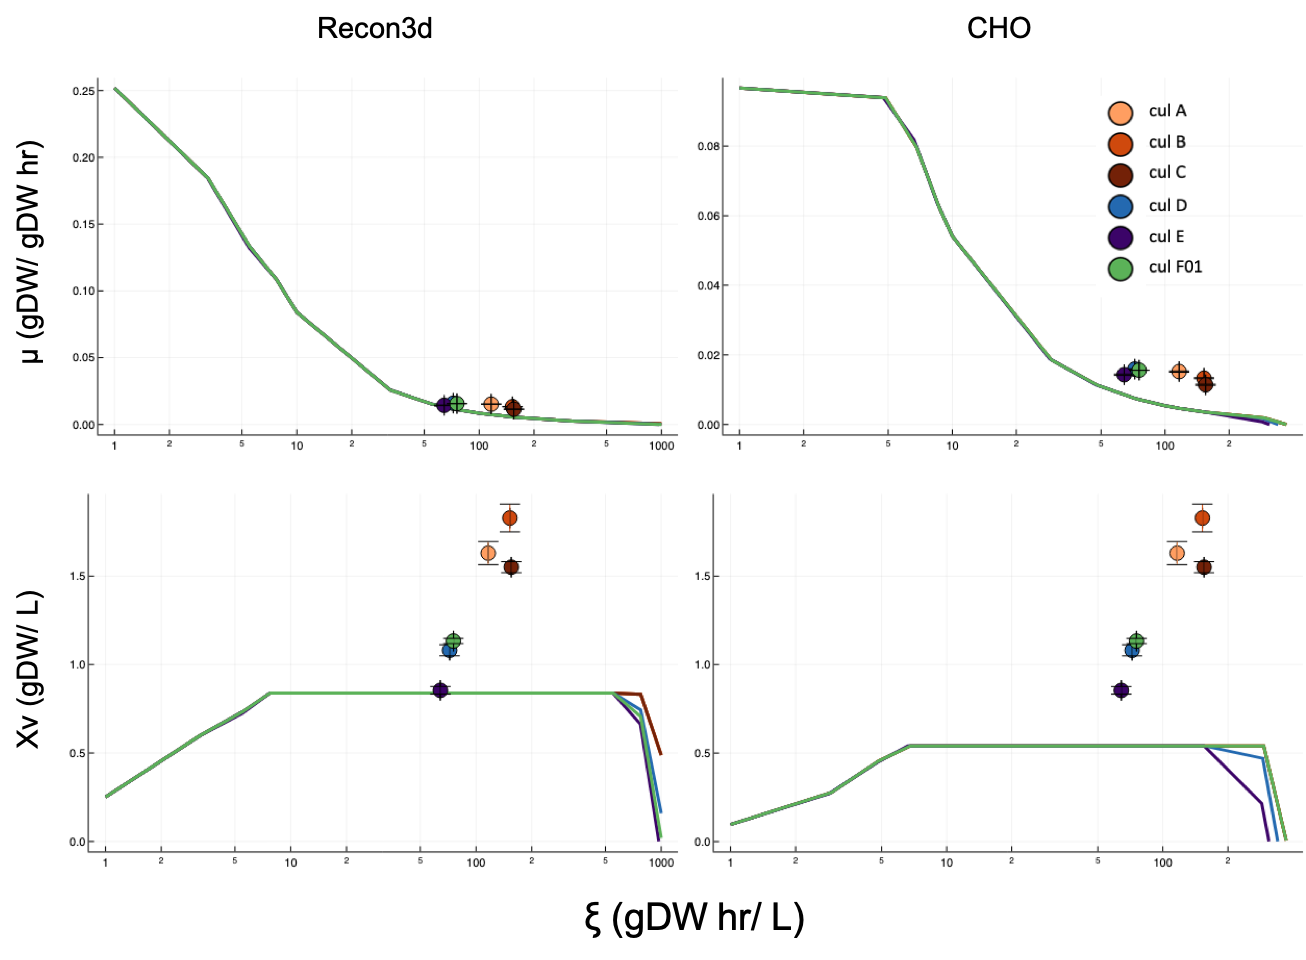
\includegraphics[scale = 0.5]{low_medium_1}
		\caption{FBAwMC results showing the growth rate, $\mu$, and the viable cell density, $Xv$, dependence of $\xi$ for the six steady states. The solid lines represent the model predictions and the colored points show the experimental results. The model data was obtained for feed mediums with low (Recon3D) and zero (CHO) concentration of phosphatidylethanolamine}
		
	\end{figure}
	
	\begin{figure}[h]
		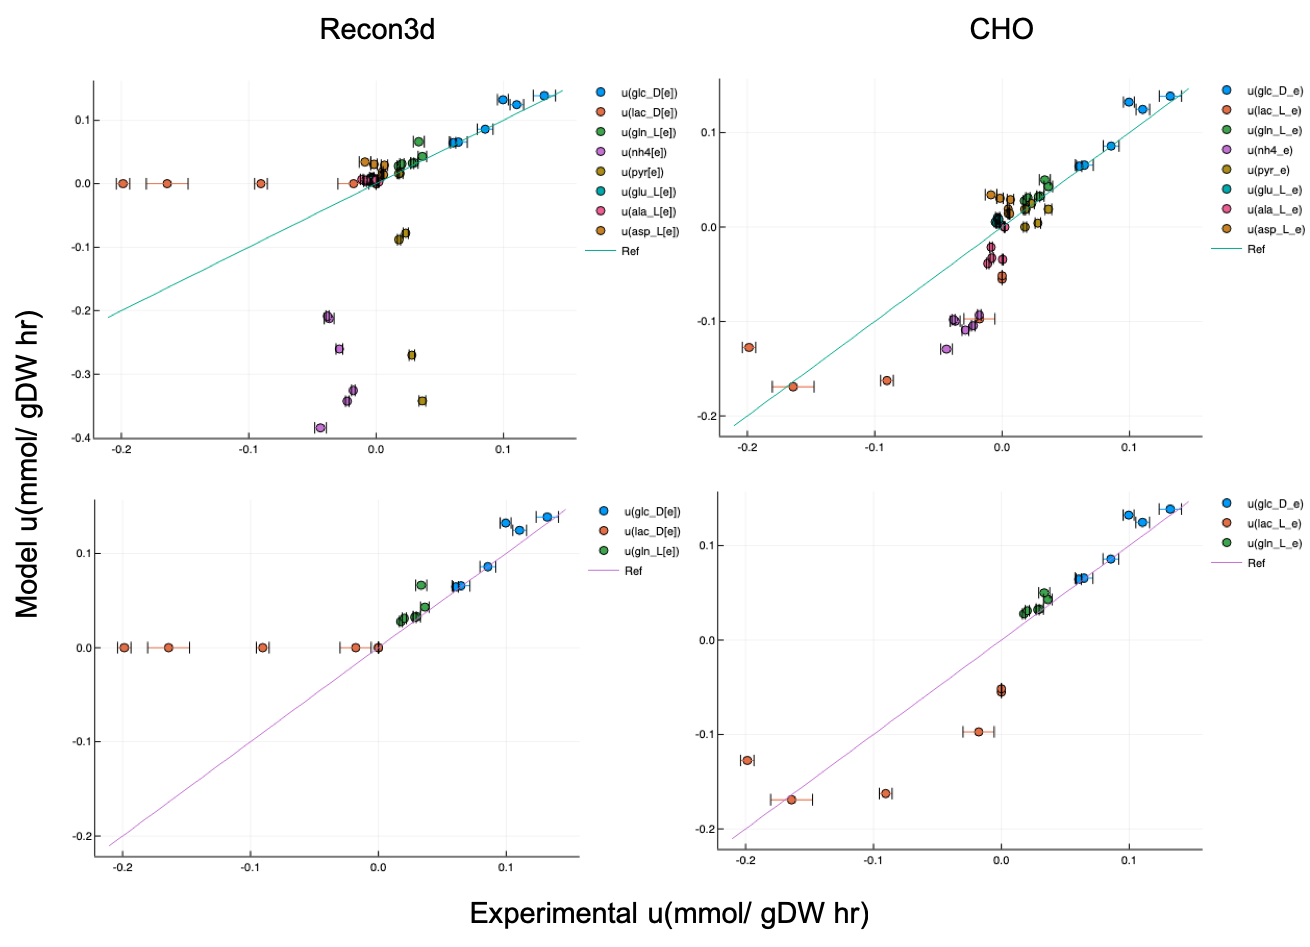
\includegraphics[scale = 0.5]{low_medium_2}
		\caption{Correlations of all the experimental uptakes, upper graphs, and a selected subset, inferior graphs, respect to the predicted value from FBAwMC with low (Recon3D) and zero (CHO) concentration of phosphatidylethanolamine.}
		
	\end{figure}
	
	\begin{figure}[h]
		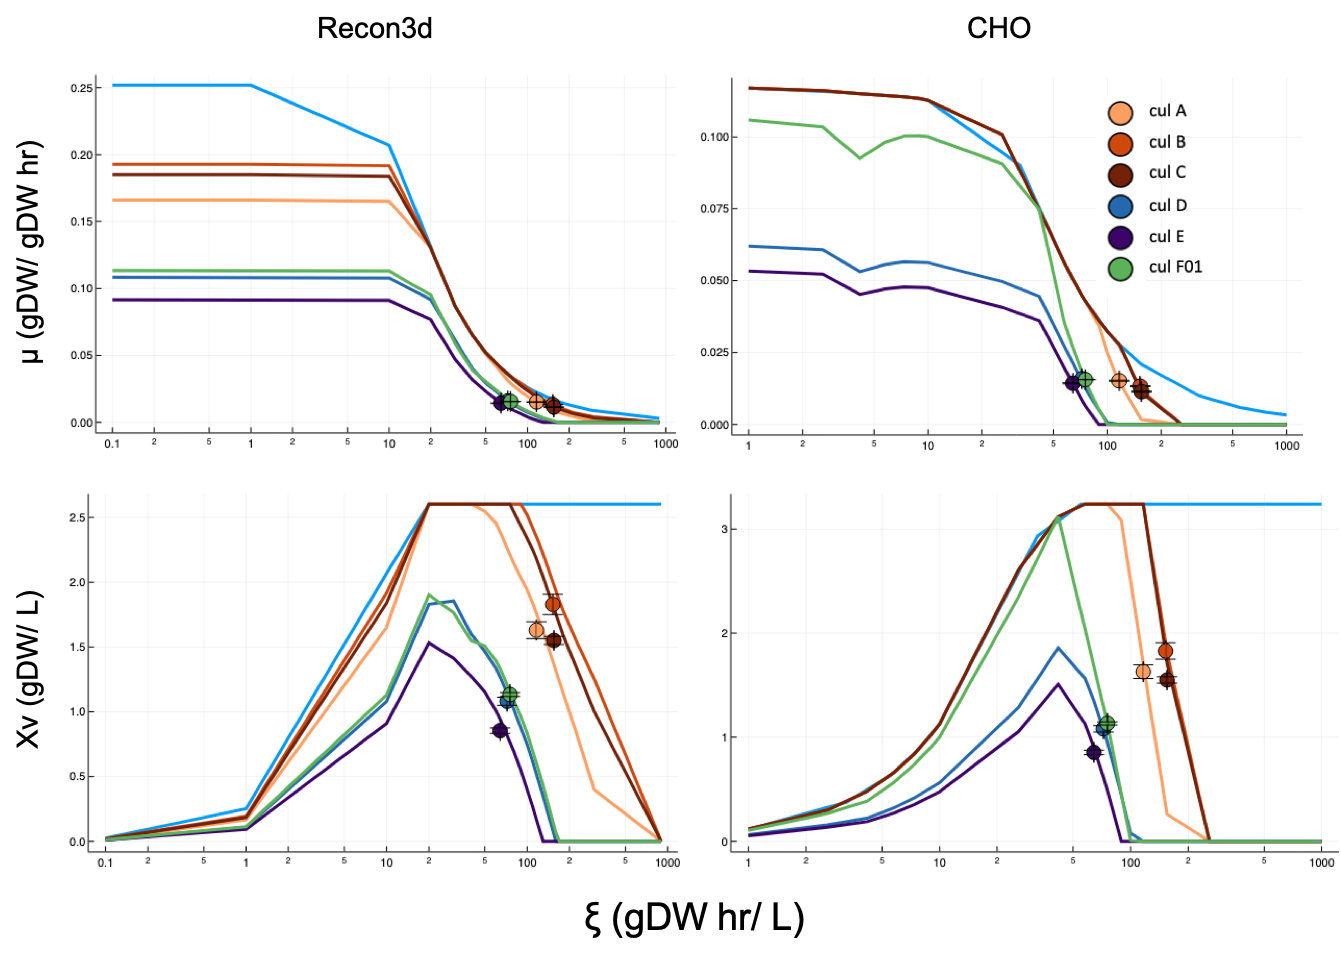
\includegraphics[scale = 0.5]{rich_medium_1}
		\caption{EP and FBA results showing the growth rate and the viable cell density dependence of $\xi$ for the six culture conditions. The solid lines represent the model predictions and the color points show the experimental results. FBA results are shown as the solid light blue line. $EP$ $\beta$ parameters was chosen, for each culture, so that the experimental $\mu$ coincides with the predicted $\mu$}
		
	\end{figure}
	
	\begin{figure}[h]
		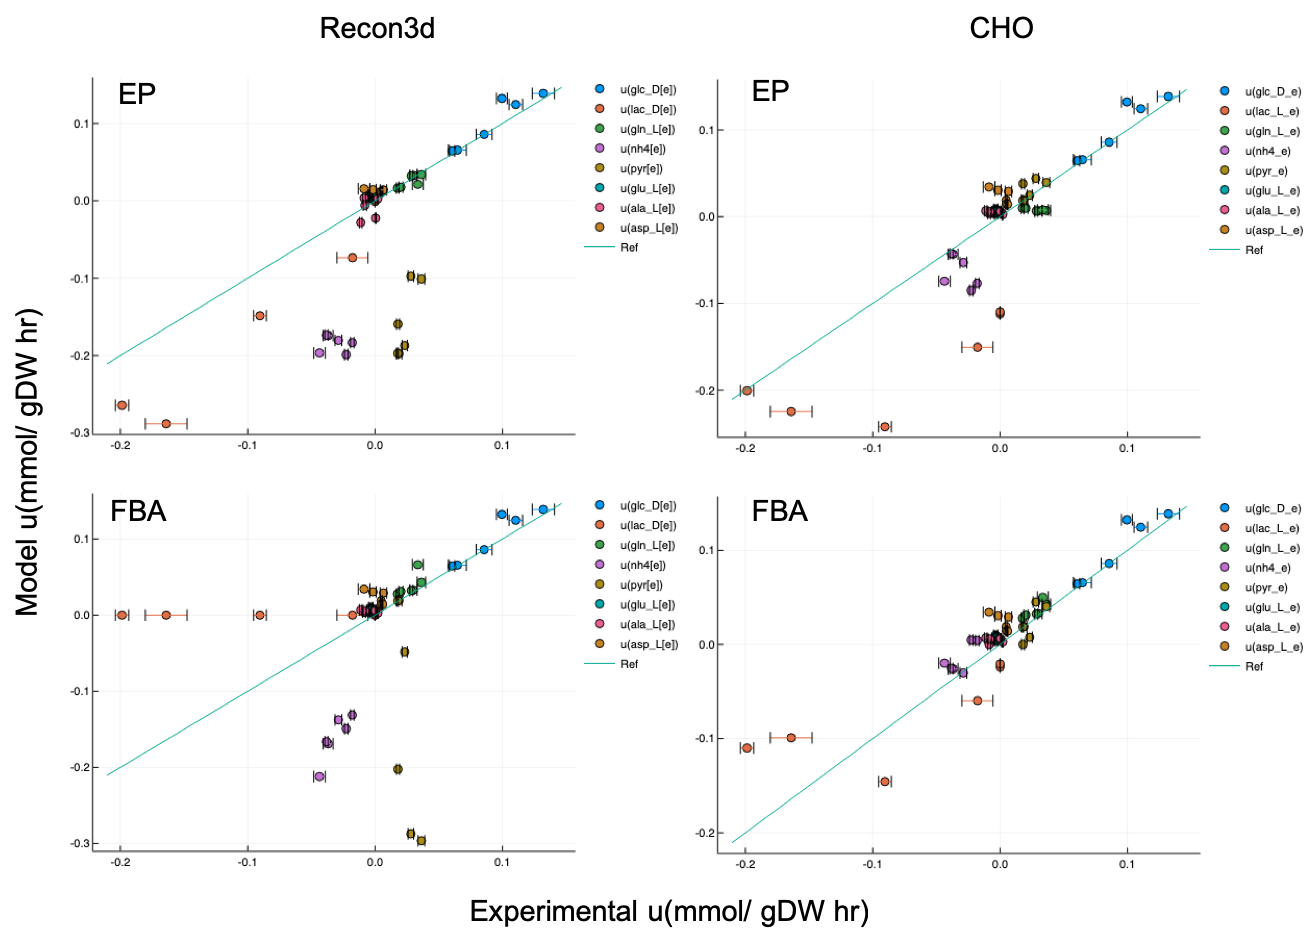
\includegraphics[scale = 0.5]{rich_medium_2}
		\caption{Correlations of all the experimental uptakes compared with the predicted value from EP and FBA for GEMs with high concentration of phosphatidylethanolamine.}
		
	\end{figure}
	
	\begin{figure}[h]
		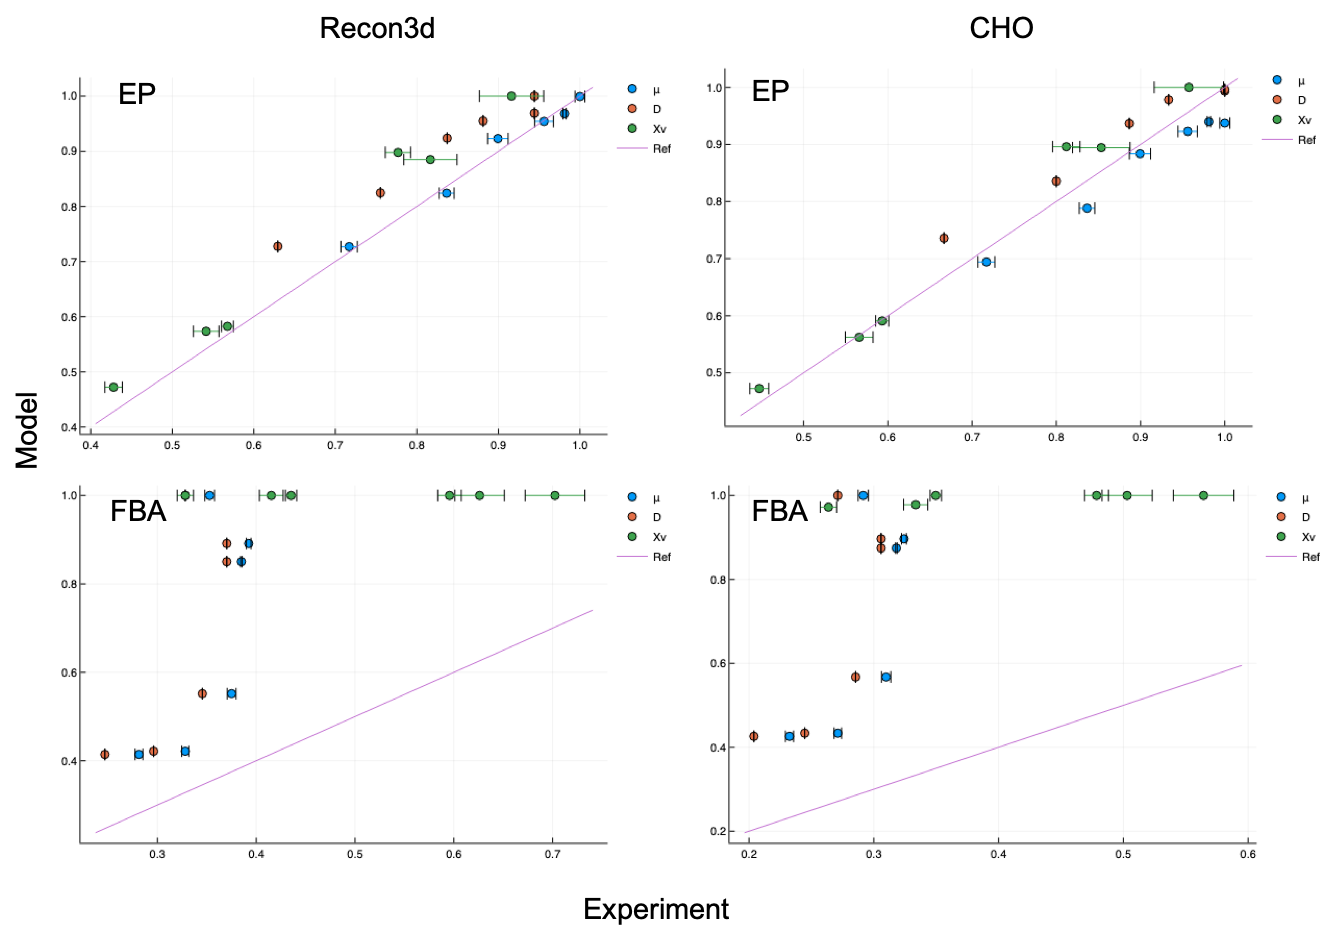
\includegraphics[scale = 0.5]{rich_medium_3}
		\caption{Normalized correlations of the experimental $\mu$, $D$ and $Xv$ compared with the predicted value from EP and FBA for GEMs with high concentration of phosphatidylethanolamine.}
		
	\end{figure}
	
\end{document}

